\section{Loss Function}
Pixel-wise loss functions such as MSE struggle to handle
the uncertainty inherent in recovering lost high-frequency
details such as texture. Minimizing the MSE encourages finding pixel-wise averages of plausible solutions which are typically overly-smooth and thus have poor perceptual quality. We illustrate the problem of minimizing MSE in Figure \ref{mse and gan comparison} where multiple potential solutions with high texture details are averaged to create a smooth reconstruction.

\begin{figure}[h!]
\centering
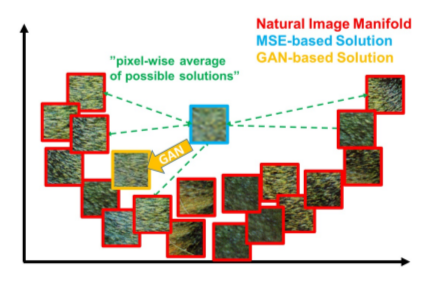
\includegraphics[scale=0.5]{mse_and_gan_comparison.png}
\caption{Illustration of patches from the natural image
manifold (red) and super-resolved patches obtained with
MSE (blue) and GAN (orange). }
\label{mse and gan comparison}

\end{figure}

\subsection{Perceptual Loss Function}
The definition of the perceptual loss function $\l^{SR}$ is critical for the performance of the generator network. We use the perceptual loss as the weighted sum of a content loss $\l_X^{SR}$ and an adversarial loss component as:
\begin{equation}
l^{SR}=l_X^{SR}+10^{-3}l_{Gen}^{SR}
\end{equation}
$\l_X^{SR}$ $\rightarrow$ Content Loss\\ \\
$10^{-3}l_{Gen}^{SR}$ $\rightarrow$ Adversarial Loss\\

\subsubsection{Content Loss}
The pixel-wise MSE loss is calculated as:
\begin{equation}
l_{MSE}^{SR}=\frac{1}{r^2WH}\sum_{x=1}^{rW}\sum_{y=1}^{rH}(I_{x,y}^{HR}-G_{\theta_{G}}(I^{LR})_{x,y})^2
\end{equation}
This is the most widely used optimization target for image
SR on which many state-of-the-art approaches rely. However, while achieving particularly high PSNR,solutions of MSE optimization problems often lack high-frequency content which results in perceptually unsatisfying solutions with overly smooth textures.\\ \\
Instead of relying on pixel-wise losses we use a loss function that is closer to perceptual similarity. We define the VGG loss based on the ReLU activation layers of the pre-trained 19 layer VGG network. With $\phi_{i,j}$ we indicate the feature map obtained by the $j^{th}$ convolution (after activation) before the $i^{th}$ maxpooling layer within the VGG19 network, which we consider given. We then define the VGG loss as the euclidean distance between the feature representations of a reconstructed image $G_{\theta_{G}}(I^{LR})$ and the reference image $I^{HR}$:

\begin{equation}
l_{VGG/i.j}^{SR}=\frac{1}{W_{i,j}H_{i,j}}\sum_{x=1}^{W_{i,j}}\sum_{y=1}^{H_{i,j}}(\phi_{i,j}(I^{HR})_{x,y}-\phi_{i,j}(G_{\theta_{G}}(I^{LR}))_{x,y})^2
\end{equation}
Here $W_{i,j}$ and $H_{i,j}$ describe the dimensions of the respective feature maps within the VGG network.

\subsubsection{Adversarial Loss}
In addition to the content losses described so far, we have to add the generative component of our GAN to the perceptual loss. This encourages our network to favour solutions that reside on the manifold of natural images, by trying to fool the discriminator network. The generative loss $l_{Gen}^{SR}$ is defined based on the probabilities of the discriminator $D_{\theta_{D}}(G_{\theta_{G}}(I^{LR}))$ over all training samples as:
\begin{equation}
l_{Gen}^{SR}=\sum_{n=1}^{N}-logD_{\theta_{D}}(G_{\theta_{G}}(I^{LR}))
\end{equation}
Here, $D_{\theta_{D}}(G_{\theta_{G}}(I^{LR}))$ is the probability that the reconstructed image $G_{\theta_{G}}(I^{LR})$ is a natural HR image. For better gradient behaviour we minimize $-logD_{\theta_{D}}(G_{\theta_{G}}(I^{LR}))$ instead of $log[1-D_{\theta_{D}}(G_{\theta_{G}}(I^{LR}))]$.
 
 